\documentclass[a4paper,11pt]{article}
\usepackage[margin=2cm]{geometry}
\usepackage{anysize}
\usepackage[pdftex]{graphicx}
\usepackage{url}
\usepackage{listings}
\usepackage{textcomp}
\usepackage{wrapfig}
\usepackage{color}
\usepackage{fancyhdr}
\usepackage[nodayofweek]{datetime}
\usepackage[small,compact]{titlesec}
\usepackage[pdfborder=0]{hyperref}
\longdate

\setlength{\parskip}{10pt} 
\setlength\parindent{0pt}
\pagestyle{fancyplain}
\fancyhf{}
\lhead{\fancyplain{}{M.Sc.\ Group Project Report}}
\rhead{\fancyplain{}{\today}}
\cfoot{\fancyplain{}{\thepage}}


\title{Twitter for traffic\\\Large{--- Final Report ---}}
\author{Porfyrios Vasileiou, Marianna Polatoglou, Afxentios Hadjiminas,\\
        Panagiotis Tsirigotis, Hanguang Zhou, John Flanagan.\\
       \{pv311, mp1911, ah2411, pt1111, hz511, jf311.\}@doc.ic.ac.uk\\ \\
       \small{Supervisors: Dr.\ Emil Lupu, Dr.\ Alessandra Russo, Luke Dickens}\\
       \small{Course: CO533, Imperial College London}
}



%Report details http://www.doc.ic.ac.uk/~cristic/teaching/MScGroupProj/

\begin{document}
\maketitle

\section{Introduction}
	Twitter for traffic aims to provide the mobile user with an application for assessing traffic disruptions as they evolve. To provide this insight, the application will present the user with curated traffic disruptions augmented with social knowledge of the event harvested from a social network. In addition to this curated list of traffic disruptions, Twitter for traffic will also extract clusters of disruption reports from social networks to identify new disruptions.

To successfully achieve the project goals, the development will encompass an understanding from many areas of computer science. Aspects of this project include data mining, social network analysis, mobile application development, document classification and geographical information systems. Analysing the social and curated datafeeds to identify new disruption events will be a particularly interesting undertaking. From the onset there are many unknowns relating to the data analysis, relating to the quantity of traffic related messages and quality of the content. 


\section{Specification}
	

\subsection{Server}

\subsection{Client}


\section{Design}
	
\subsection{System overview}
	\begin{center}
	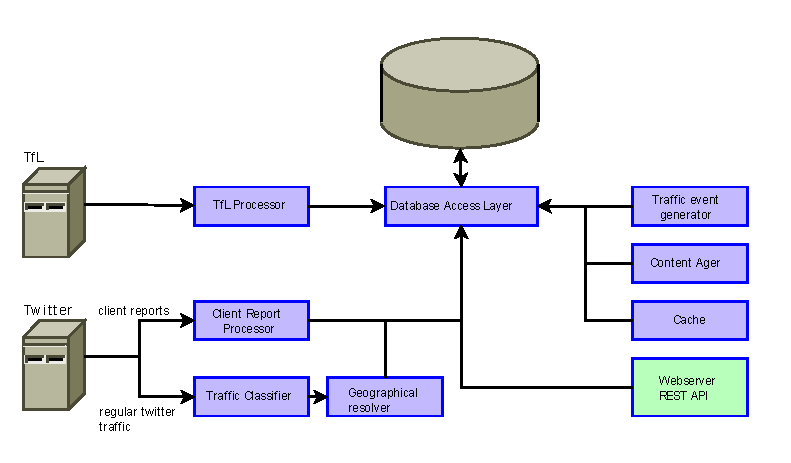
\includegraphics{images/high_level_system_arch.pdf}
	\end{center}
\subsection{Server}
  
\subsubsection{Data acquisition}
\subsubsection{Data analysis}
\subsubsection{Storage}
\subsubsection{Interface}


\subsection{Client}
  \begin{figure}[htb]
\centering
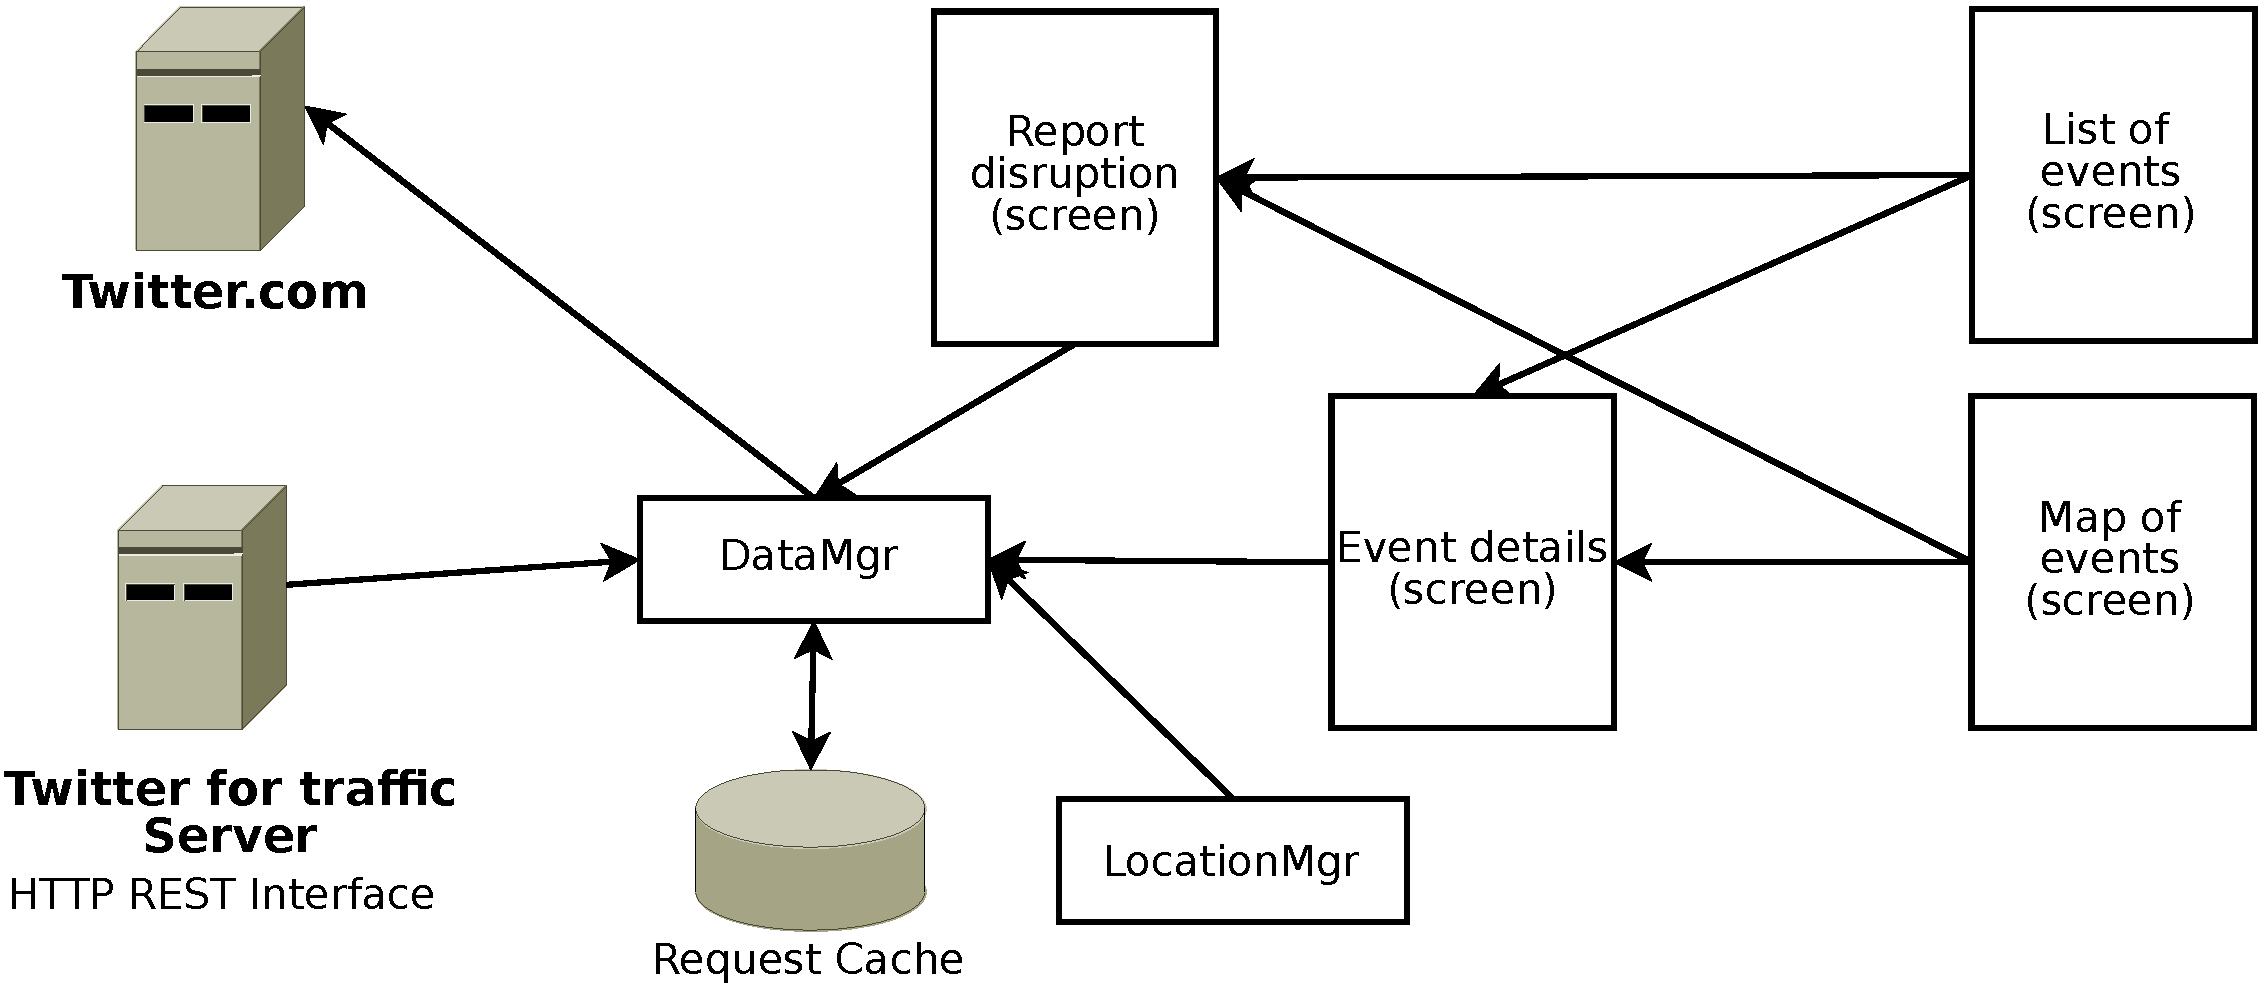
\includegraphics[width=0.9\textwidth]{images/design/client/client_high_level_layout.pdf}
\caption{High level client design}
\label{fig:client_design}
\end{figure}



\subsubsection{User interface}
\subsubsection{Request caching}




\section{Methodology}
	\subsection{Development approach} 
To begin identifying an appropriate development methodology, it was necessary to firstly understand 
the project requirements. The project requirements and features were agreed over a number of 
meetings with the primary stakeholders.

The two most preferred development methodologies were 
Scrum and XP(Extreme Programming) which are both Agile methodologies. Scrum is an agile project management technique that focuses more 
on the management of software development projects. The product is completed in a series of one to 
four week iterations, or sprints as they are called. Before each sprint, a planning meeting is held 
to determine which features will be implemented during that sprint. Similarly, XP is an agile 
methodology which is designed for small, co-located teams aiming to get quality and productivity as 
high as possible. It does this through the use of rich, short, informal communication paths with 
emphasis on skill, discipline and understanding at the personal level, minimizing all intermediate 
work products. 

It was decided amongst the group that combining characteristics form both methods 
would be the most beneficial way, merely because they are complementary. Scrum focuses on the project management 
whereas XP on the programming part.\cite{ScrumXP}

Managing efficiently the development lifecycle of the project was a very 
important task for the team to work properly. Meetings with the supervisor took place each week 
where the project progress was thoroughly discussed as well as more feasible features to be 
implemented. In addition, various issues were constantly being brought up in order to provide solutions. Except from 
the meetings with the supervisor, the team had its own weekly meeting for keeping up with what 
everyone has been doing for the last week. New tasks were also assigned to members of the team. For 
every meeting an agenda was stored in an online document containing information about the team 
members absent, location, action items and topics to be discussed. In the end of the meeting tasks 
were assigned, managed or archived using an online visual board, similar to the Scrum Board, to 
encourage a more agile development.

As regards to the XP approach, it was proved that adopting 
some of its techniques would significantly improve the development process. More specifically, pair 
programming was effectively put in use. Team members where working in pairs whenever possible to 
develop a single feature. Additionally, XP promotes test-driven development. As mentioned in the 
first report, testing would be rather difficult due to the nature of the project being partly 
research based. However, essential tests were implemented in the server to validate the classifier 
as well as blackbox tests for the correctness and responsiveness of the rest API server. 

Throughout the development, various technologies had to be used and implemented. According to each 
members skills these elements were divided in such ways to effectively use the members previous 
experience. The team was also distributed to different design aspects of the project; however, more on the 
team structure will be discussed further on.

Lastly, for achieving parallel development between the mobile client application and the server, 
a mock server API was created, as mentioned in earlier reports that was accepting http requests and 
was returning static data sets to the client. 

\subsection{Testing} 
\subsubsection{Classifier Evaluation} 
Machine learning algorithms induce classifiers that depend on the training set, and there is a need for evaluation and statistical testing to assess the expected error rate of a classification algorithm, and even compare the expected error rates of two classification algorithms to be able to say which one is better. Evaluation can also be used as a guide for future improvements on the model. In order to evaluate the classifier several techniques have been used. The first technique is to generate a test set of tweets which their labels are already known. This test set has to be distinct from the train set which has been used to train the classifier. Afterward this test set is being classified by the classifier and the labels that it decides are being compared with their correct labels. The second technique is to calculate the accuracy of the classifier which measures the percentage of inputs in the test set that the classifier correctly labelled. To accomplish this, the build-in function of the package NLTK \emph{nltk.classify.accuracy()} has been used.

Additionally some more techniques have been implemented in order to get more
accurate evaluations and avoid possible `overfitting'. Note that there is a chance the classifier will become more accurate in the train set and less accurate in the test set with some parameter changes. This is when we have reached an "overfitting" to the train set. The first of these methods is the K-Fold Cross Validation. The dataset is split each time into K equally sized subsets, training and testing datasets, and then in n-th iteration (n=1..k) the n-th subset(testing set) is used for testing the classifier that has been built on all other remaining subsets. To present the result of this method the Confusion Matrix, which is a visualization tool typically used to present the results attained by a learner, has been created. Each column of the matrix represents the instances in a predicted class, while each row represents the instances in an actual class. Thus, the diagonal entries indicate labels that were correctly predicted, and the off-diagonal entries indicate errors. One benefit of a confusion matrix is that it is easy to see if the system is confusing two classes.

Finally, the Precision and Recall Rates can be calculated in order to ensure the results from the previous method. The recall and the precision can be derived from the confusion matrix by applying the following formulas:

\[ Precision\textsubscript{A} = tp\textsubscript{A}/(tp\textsubscript{A}+e\textsubscript{BA}+e\textsubscript{CA}) \]

\[ Recall\textsubscript{A} = tp\textsubscript{A}/(tp\textsubscript{A}+e\textsubscript{AB}+e\textsubscript{AC}) \]

Where the values "tp" and "e" are the elements of the confusion matrix as it can been seen on the figure~\ref{fig:confisionMatixCalc}.

\begin{figure}[h]
\begin{center}
\begin{tabular}{| l || c | c | c | }
    \hline
        & A & B & C  \\ \hline \hline
        A & tp\textsubscript{A} & e\textsubscript{AB} & e\textsubscript{AC} \\ \hline
        B & e\textsubscript{BA }& tp\textsubscript{B} & e\textsubscript{BC} \\\hline
        C & e\textsubscript{CA} & e\textsubscript{CB} & tp\textsubscript{C} \\\hline
    \end{tabular}
	\caption{A simple confusion matrix}
    \label{fig:confisionMatixCalc}
\end{center}
\end{figure}

While recall and precision rates can be individually used to determine the quality of a classifier, it is often more convenient to have a single measure to do the same assessment. The F\textsubscript{1} measure combines the recall and precision rates in a single equation:

\[ F\textsubscript{1} = 2*\frac{precision*recall}{precision+recall} \]

Because the labelled data was consisting of 1500 traffic tweets and 14505 non-traffic tweets, two different trainings and evaluations have been integrated. 

Firstly, the classifier was trained with 1000 traffic and 1000 non-traffic tweets. Then it was tested with 500 traffic and 500 non-traffic tweets. The metrics for this training are the following. 

Accuracy of the classifier:   0.87\\

Traffic precision:\hspace{15.5 mm}              0.842592592593\\
Traffic recall:\hspace{21.2 mm}                             0.91\\
Traffic F-measure:\hspace{12.8 mm}             0.875\\

Non-Traffic precision:\hspace{7.2 mm}        0.902173913043\\
Non-Traffic recall:\hspace{13 mm}            0.83\\
Non-Traffic F-measure:\hspace{4.6 mm}       0.864583333333\\

\begin{figure}[h]
\begin{center}
    \begin{tabular}{| l || c | c | }
    \hline
          & Non-Traffic & Traffic \\ \hline \hline
         Non-Traffic & 41.5\% & 8.5\% \\ \hline
         Traffic & 4.5\% & 45.5\% \\ \hline
    \end{tabular}
    \caption{Confusion Matrix with 1000 traffic and 1000 non-traffic tweets.}
    \label{fig:confusionMatrix1}
\end{center}
\end{figure}	

Secondly, the classifier was trained with 1000 traffic and 9670 non-traffic tweets. Afterward it was tested with 500 traffic and 4835 non-traffic tweets. The metrics for this training are the following. 

Accuracy of the classifier:   0.862605435801

Traffic precision:\hspace{15.5 mm}            0.401019541206\\
Traffic recall:\hspace{21.2 mm}               0.944\\
Traffic F-measure:\hspace{12.8 mm}         0.562909958259\\

Non-Traffic precision:\hspace{7.2 mm}         0.993265993266\\
Non-Traffic recall:\hspace{13 mm}           0.854188210962\\
Non-Traffic F-measure:\hspace{4.6 mm}         0.918492160569\\

\begin{figure}[h]
\begin{center}
    \begin{tabular}{| l || c | c | }
    \hline
          & Non-Traffic & Traffic \\ \hline \hline
        Non-Traffic & 77.4\% & 13.2\% \\ \hline
        Traffic & 0.5\% & 8.8\% \\ \hline
    \end{tabular}
    \caption{Confusion Matrix with 1000 traffic and 9670 non-traffic tweets.}
    \label{fig:confusionMatrix1}
\end{center}
\end{figure}
	
It can been observed from the confusion matrices, with the first training the classifier has been achieved a rather bad accuracy since 19\% of the non-traffic tweets are being classified wrong and 9\% of the traffic tweets are being classified wrong. On the other hand, with the second training the traffic tweets error has been almost halved to 5\% resulting a more accurate classification for the traffic tweets even if the global accuracy dropped by 1\%. That means the classifier may classified some traffic tweets as non-traffic but it classified much less non-traffic tweets as traffic. Note that all the above results have been taken after the implementation of the normalization. During the first evaluation, before the pre-processing, the accuracy of the classifier was 77\%. However after the application of the normalization�s techniques the accuracy has been increased by 10\%!

As it has been mentioned before, a strong motivation for the creation of this project was the previous work of Dr. Luke Dicken in the same field. Having that in mind, it has been considered necessary to compare the accuracy of the classifier and the efficient of the server with his work. So in addition to the previous evaluation results, several metrics have been calculated in order to find the efficient of the classifier and the server. Those metrics are being presented in the figures below.

\begin{figure}[h]
\begin{center}
    \begin{tabular}{| c | c | c | }
    \hline
        Total Number of Tweets  & Non-Traffic & Traffic \\ \hline 
        71036 & 68096(95.86\%) & 2940(4.14\%) \\ \hline
    \end{tabular}
    \caption{Comparison of Traffic and Non-Traffic Tweets.}
    \label{fig:metrics1}
\end{center}
\end{figure}
	
\begin{figure}[h]
\begin{center}
    \begin{tabular}{| c | c | c | }
    \hline
        Geo-Tagged  & Geo-Tagged Genuine & Geo-Tagged from the 
Geolocation Resolver \\ \hline 
        314(10.68\%) & 136(4.63\%) & 178(6.05\%) \\ \hline
    \end{tabular}
    \caption{Tweets with geolocation from the 2940 traffic tweets.}
    \label{fig:metrics2}
\end{center}
\end{figure}


\begin{figure}[h]
Overall inferred rates:
\begin{center}
    \begin{tabular}{| l || c | c | c |}
    \hline
        & Filtered & Traffic & Geo-Tagged and Traffic\\ \hline \hline
        each minute & 13.3 & 0.5 & 0.06 \\ \hline
		each 5 mins & 66.7 &  2.7 & 0.3 \\ \hline
		each hour & 800 & 32.7 & 3.5 \\ \hline
    \end{tabular}
    \caption{Averages are over total 5400 minutes (90 hours) of up-time.}
    \label{fig:metrics3}
\end{center}
\end{figure}


\subsubsection{Functional/Integration Testing}
One of the most important parts of the project was the server API interface. A lot of requests will 
be coming from the mobile application and it must be confirmed that the server interface can handle 
them but also return the expected results using the expected format. In order to test the server 
interface the Apache JMeter desktop application was used. This software is designed to load test 
functional behaviour and measure the performance of static and dynamic recourses. Using JMeter 
proved to be a very effective way to test the servers interface. Various test plans where created 
testing every GET or POST request available to use through the API. These plans where created for 
both the server and the mock server that are running on ports 55004 and 55003 accordingly. More 
tests were implemented to ensure that the server was returning the correct messages and response 
codes when it was encountering an error. In addition, invalid requests to the server had also been 
checked for error handling and if the error messages were displayed correctly into the screen. For 
each request, the content-type was also checked if it evaluates as JSON. This process was really 
helpful because it was very easy later on to check whether new features implemented or code 
refactoring were actually breaking the API. All the test plan configuration settings have been saved 
in the project repository as a .jmx file. 

\subsubsection{Unit Testing} 



\section{Group Work}
	\subsection{Team Structure} 
Before starting working on the project, the team structure had to be defined. Most importantly, we had to 
agree who would be the leader of the group whose main responsibility was coordinating the tasks amongst the 
team members. At the early stages of the project, all features were researched in order to 
determine their feasibility and to estimate the amount of work required for each one. Next, according to 
each members previous experience and expertise, the team was divided into 3 subgroups, each one assigned to 
a different aspect of the project. Only one person was responsible for designing the client application, while
we provisioned the team manpower to the server. Two members were allocated to creating and training 
the classifier and two more focused on the implementation of the server. The last person was rotating through 
all the aspects of the project, providing help when needed. Every team member was expected to contribute 
at least 10 hours per week on this group project.\\ 

\subsection{Collaboration Tools} 
Project management is a vital part of any project. There exist a series of tools that enable effective team 
collaboration during a project. One of these tools is \emph{Trello} which gives access to a visual board 
that displays the ongoing tasks. This concept is very similar to the Scrum board. All these tasks 
are represented as cards with labels, priorities and deadlines assigned to 
team members. In this visual board we have the lists for separating the tasks such as `To Do', `Started', `Review' and `Done this week'. 
Additionally, six labels were created with different colours to identify their kinds of tasks like data, 
documentation, server, android app, text analysis and meeting preparation. Future tasks were 
discussed at the weekly group meeting and assigned to the `To Do' list. A team member who started a task that he was responsible of, 
would drag this card to the `Started' list to inform the rest group members that this task was currently being processed. 
After a task was finished, the card was moved to the `Review' list so other members would evaluate it. 
On every group meeting, reviewed tasks were transferred to the `Done this week' list and in the end of the meeting they were
archived.\\ 
Another tool that has been used for this project was Github. Github is used as our revision control system to manage 
the source-code and documentation. It enables multiple team members to work on a set of files, 
ensuring that changes will not get lost. Other features include version tracking, verifiable histories, integration with deployment, 
test and code review systems and the ability to add rules to enforce corporate policy and process. \\
When a team member makes changes to a file in the project, his next step is to commit it and push it to the repository. 
This updates the state of the project and the other team members can pull and receive the updated project repository. 
Github stores the history of all the changes so that individuals can compare or revert 
to previous versions of the project. Furthermore, Github provides a `Wiki' feature that enables team members 
to add description or instructions for specific components that are implemented in the project.\\
From the beginning of the project it was agreed that all data will exist outside of the repository. This was enforced by 
policy and by using a `.gitignore' file of the repository to list file types to be not tracked.


% A repository called 'Twitter for Traffic' is created in 
% Github. The project is divided into several parts. We create a 'classifier' file for data mining and 
% 'data\_acquisition' file to retrieve tweets and TfL data. 'mobile\_client' folder is built for 
% Android application development. 'mock\_server' and 'server' folders are platform which is providing 
% and processing data for mobile client. A folder called 'scrapbook' is created for each members to 
%store source codes and test each unit function.

	
\section{Final Product}
	\subsection{Achieved goals and difficulties}
The specifications and which of them were implemented or not is described in
Section 2. All the features from the minimum specifications were imlemented
fully. Also, there were features that were not in the specifications and were
implemented nonetheless.

A profanity checker was included, as stated in Section 4.2.1, to check if the social data included any
cursing words. Every time a tweet is processed before entering the database
there is a profanity check and it is marked accordingly. By default the
application does not use the profanity checker, but the user can enable it from
the settings.

Soundex algorithm was implemented as well, as stated in Section 4.2.2, in order to enhance the possibility to identify
a location just from the text of a tweet. This algorithm understands
misspelled words, and so gives the ability to search for street names that may
be mistyped.

The reasons some features were not included in the final project is
that there were some difficulties that could not be overcome, or the priorities
changed.
The reasons they were not implemented are described below:

\emph{Identify traffic disruptions from Twitter}

The reason that this feature could not be included is that the traffic tweets
for a small timeslice are too few to get results from the clustering described
in Section 7.1. The feature is still implemented, but the data used to test
were in a timeslice of an hour and using data that were not specifically about
traffic. This means that a new cluster we may find might also indicate an
event that is irrelevant to traffic. Nonetheless, this should prove very useful
in the future.

\emph{Enhance clustering algorithm}

This feature could not be included in the product of this project because we
could not implement clustering to work in real time, as described in the
previous feature that was not implemented.

\emph{Present tweets on the map}


\pagebreak

\section{Appendix}
	\subsection{Included libraries}
    \subsubsection{Server}

\begin{description}
    \item[Flask] \url{http://flask.pocoo.org/} \hfill \\
        Provides a REST API used for the server.
    \item[pg8000] \url{http://pybrary.net/pg8000/} \hfill \\
        Provides functions used for PostgreSQL.
    \item[NLTK] \emph{Natural Language Toolkit} \url{http://code.google.com/p/nltk/} \hfill \\
        Provides tools used for the classifier.
    \item[python-twitter] \url{http://code.google.com/p/python-twitter/} \hfill \\
        Provides Twitter search functions.
    \item[tldextract] \url{http://pypi.python.org/pypi/tldextract/0.2} \hfill \\
        Finds a domain name from a url.
    \item[googlemaps] \url{http://pypi.python.org/pypi/googlemaps/} \hfill \\
        Provides reverse geocoding from Google Maps.
    \item[OSGB36toWGS84] \url{http://hannahfry.co.uk/2012/02/01/converting-british-national-grid-to-latitude-and-longitude-ii/} \hfill \\
        Module providing conversion between the national British grid coordinates and longitude, latitude coordinates.
\end{description}

\subsubsection{Client}

\begin{description}
    \item[JTwitter] \emph{LGPL} \url{http://www.winterwell.com/software/jtwitter.php} \hfill \\
        Provides Twitter interface.
    \item[oauth-signpost] \emph{Apache Licence 2.0} \url{http://code.google.com/p/oauth-signpost/} \hfill \\
        Provides Oauth authentication for connecting Twitter acounts.
\end{description}


\subsection{Client user interface}
    \begin{figure}
\centering

\mbox{\subfigure{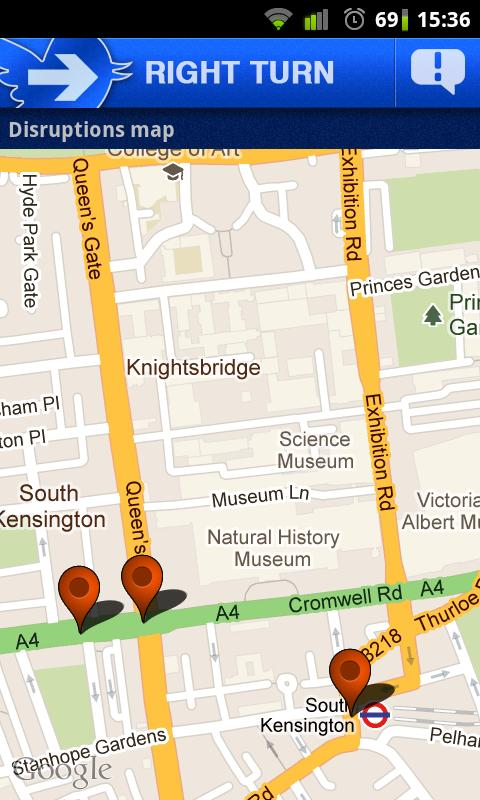
\includegraphics[width=0.4\textwidth]{images/appendix/user_interface/map_view.jpg}
\quad
\subfigure{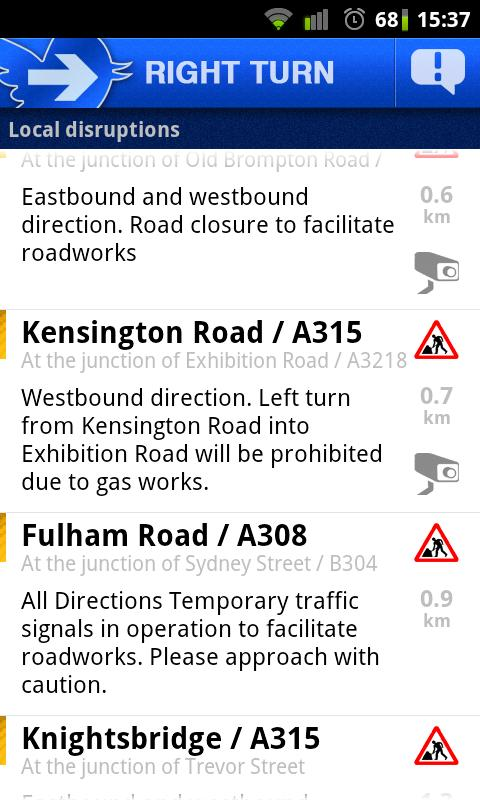
\includegraphics[width=0.4\textwidth]{images/appendix/user_interface/list_view.jpg} }}}


\mbox{\subfigure{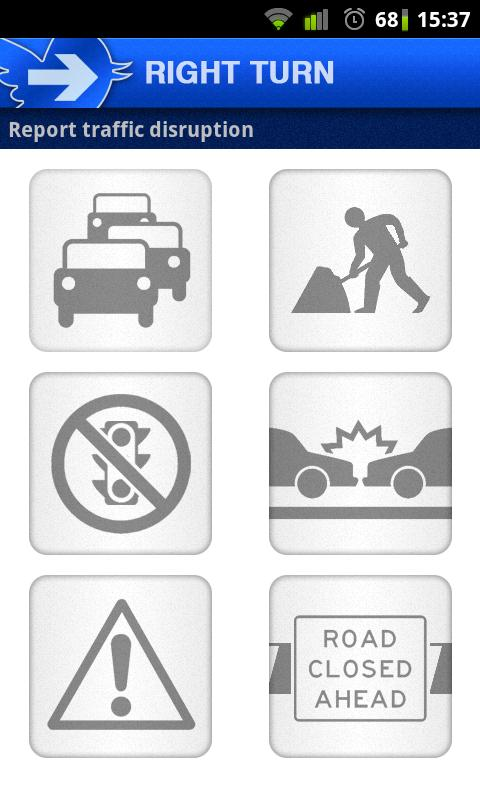
\includegraphics[width=0.4\textwidth]{images/appendix/user_interface/report_view.jpg}
\quad
\subfigure{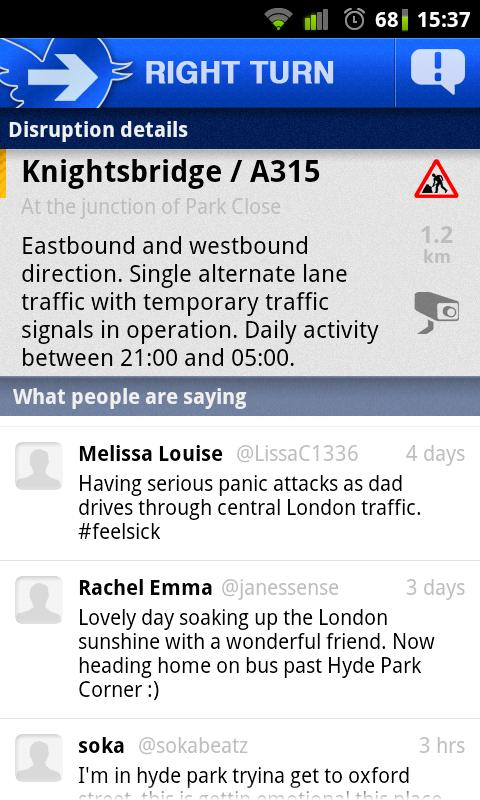
\includegraphics[width=0.4\textwidth]{images/appendix/user_interface/details_view.jpg} }}}

\caption{Examples of the implemented user interface}
\label{fig:user_interface}
\end{figure}

\begin{figure}
\centering
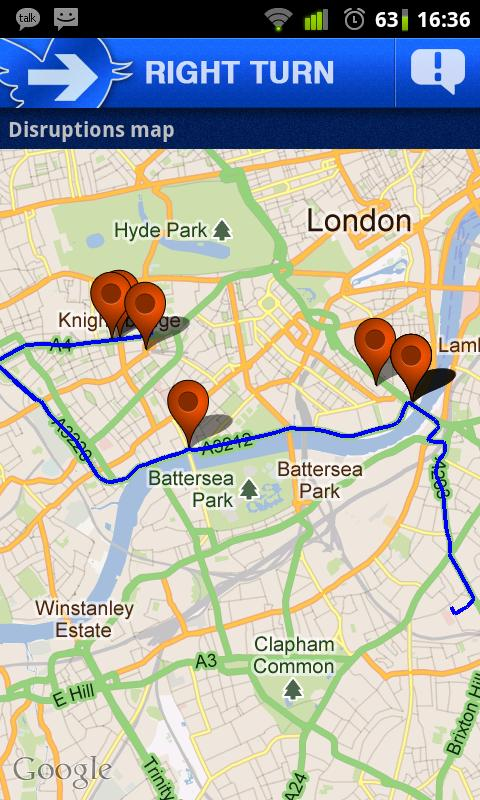
\includegraphics[width=0.45\textwidth]{images/appendix/user_interface/home_route.jpg}
\caption{Example of home route functionality}
\label{fig:home_route}
\end{figure}


\subsection{Online resources}
    \begin{description}
    \item[Github] \url{https://github.com/johnflan/Twitter-4-Traffic/} \hfill \\
        Revision control system.
    \item[Video Demonstration] \url{http://www.youtube.com/watch?v=LmWDxq2jhNI/} \hfill \\
        Video demonstration of the final product.
\end{description}


%\pagebreak	
%\section{References}
%	\vspace{-20pt}
%	\def\refname{}
%	\bibliography{references}
%	\bibliographystyle{plain}

\end{document}
